\documentclass[journal = jacsat, manuscript = suppinfo]{achemso}

\usepackage[version = 4]{mhchem}
\usepackage{graphicx}
\usepackage{mwe}

% disable symbol next to email
\makeatletter
\def\acs@author@fnsymbol#1{}
\makeatother

\SectionNumbersOn

% macros
\newcommand{\nidppe}{\ce{Ni(dppe)Cl2}}
\newcommand{\nicl}{\ce{NiCl2 $\cdot$ 6H2O}}
\newcommand{\nh}{\ce{NH3}}
\newcommand{\nanh}{\ce{Na $\cdot$ NH3}}
\newcommand{\nhbr}{\ce{NH4Br}}
\newcommand{\h}{$^1$H}
\newcommand{\p}{$^{31}$P}
\newcommand{\cdcl}{\ce{CDCl3}}
\newcommand{\niion}{\ce{Ni^{2+}}}
\newcommand{\wavenum}{cm$^{-1}$}

\newcommand{\del}{$\delta$}
\newcommand{\deleq}[1]{$\delta=#1$}

\hbadness=99999

\title{1,2-bis(diphenylphosphino)ethane (dppe) and \nidppe\ synthesis via
solvated electron reduction}

\author{David Qiu}
\affiliation{Department of Chemistry, University of Illinois at
Urbana-Champaign, 505 S Matthews Avenue, Urbana, IL, 61801}
\email{davidlq2@illinois.edu}

\begin{document}

\tableofcontents

\newpage

\section{General Considerations}

\subsection{Instruments and Materials}

\h\ NMR spectra were taken on a 60 MHz Nanalysis NMReady-60PRO tabletop NMR
instrument. \p\ NMR spectra were taken on a 400 MHz  Varian NMR spectrometer. IR
spectra were taken on a Perkin Elmer Spectrum Two FTIR spectrometer.

\textit{n}-hexane, ethanol, and \nh\ were sourced from UIUC. Diethyl ether and
Na were sourced from Fischer Chemical. Triphenylphosphine and 1,2-dichloroethane
were sourced from Acros. \nhbr\ was sourced from Oakwood Chemical.

\subsection{Hazards}

All organic solvents should be assumed to be acutely toxic, volatile, flammable,
and irritating unless otherwise noted, and should only be used within a fume
hood. \nh\ is highly volatile and flammable, is an extreme irritant to the skin
and eyes, and should be used only inside a fume hood.  Na is highly reactive
with water, and can cause severe alkali burns of the skin and eyes if direct
physical contact is made.  Triphenylphosphine is acutely toxic to the nervous
system. \nhbr\ is a respiratory irritant. Both \nicl\ and 1,2-dichloroethane are
also carcinogenic.

\section{Experimental Procedures}

\textbf{dppe synthesis\cite{handout}:} To a 500 mL round-bottom flask was
charged 200 mL of \nh, a glass-coated stir bar. A dry ice condenser connected to
a bubbler, gas inlet valve, and rubber septum were attached to the appartus. Na
(2.379 g, 0.1035 mol, 4 equiv.) was added slowly over 3 minutes. A dark blue
solution formed over 10 minutes, after which triphenylphosphine (13.55 g,
0.05166 mol, 2 equiv.) was added in 1 g portions.  This solution was stirred for
30 minutes. \nhbr\ (5.068 g, 0.05174 mol, 2 equiv.) was added.
1,2-dichloroethane (2.555 g, 0.02582 mol, 1 equiv.) was poured in and reacted
for 10 minutes. The gas inlet valve was left open to air for 1 week. The dried
reaction mixture was washed with DI water and rotary evaporated following
dilution with ethanol. The purified, milky-white dppe powder precipitated, and
was filtered out of solution and washed with ethanol.

The reaction recorded a percent yield of 118\% (12.11 g total, 10.29 g
expected). The \h\ NMR spectrum interpretation is as follows (60 MHz, \del):
7.27 ppm, 2.06 ppm (4 H, t). The \p\ NMR spectrum interpretation is as follows
(400 MHz, \del): -11.52 ppm (s). The IR spectrum interpretation is as follows
($\tilde\nu$): 2950 \wavenum\ (C--H stretch), 1400 \wavenum\ (aromatic C--C/C=C
stretch).  Aside from the presence of identified impurities and \p\ NMR
instrument artifacts, the \h\ NMR, \p\ NMR, and IR spectra are in excellent
agreement with literature values.\cite{dppenmr1, dppenmr2}

\textbf{\nidppe\ synthesis\cite{handout}:} \nicl\ (0.320 g, 1.34 mol, 1 equiv.)
was dissolved in ethanol and mixed with dppe (0.54 g, 1.34 mol, 1 equiv.). This
was allowed to react for 5 minutes. The tomato-red \nidppe\ precipitate was
filtered out and washed with diethyl ether.

The reaction recorded a percent yield of 47\% (0.33 g total, 0.71 g expected).
The \h\ NMR spectrum interpretation is as follows (60 MHz, \del): 8.01 ppm (8 H,
meta), 7.53 ppm (12 H, ortho/para), 2.12 ppm (4 H, ethane bridge). The \p\ NMR
spectrum interpretation is as follows (400 MHz, \del): $-58.23$ ppm (s). The IR
spectrum interpretation is as follows ($\tilde\nu$): 1450 \wavenum\ (aromatic
C--C/C=C stretch).  Aside from presence of identified impurities \p\ NMR
instrument artifacts, the \h\ NMR, \p\ NMR, and IR spectra are in excellent
agreement with literature values.\cite{dppeir, dppenmr1, dppenmr2}

\section{\h\ NMR Spectra}

\subsection{\h\ NMR spectrum of dppe}
\begin{figure}[H]
	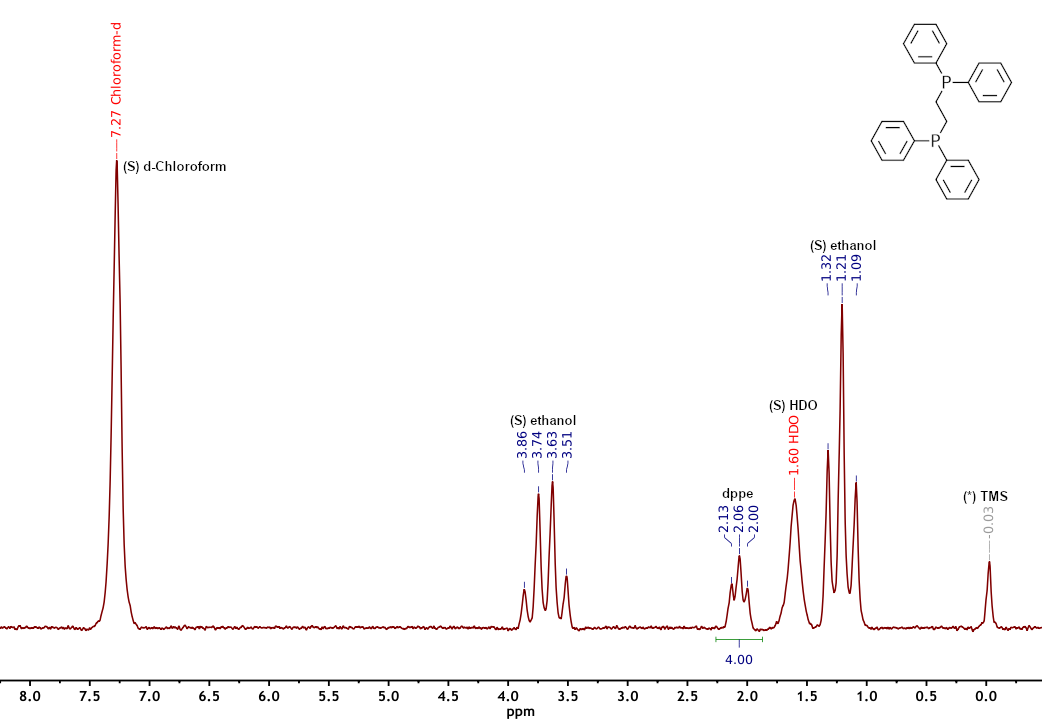
\includegraphics[width=\textwidth]{figures/dppe_hnmr}
	\caption{
		60 MHz \h\ NMR spectrum of dppe. The impurities are listed as
		follows (\del): \cite{nmrtable} 7.27 ppm (\cdcl, s), 3.58 ppm
		(ethanol, q), 1.21 ppm (ethanol, t), 1.60 ppm (HDO, s), $-0.03$
		ppm (TMS, s).
	}
\end{figure}

\subsection{\h\ NMR spectrum of \nidppe}
\begin{figure}[H]
	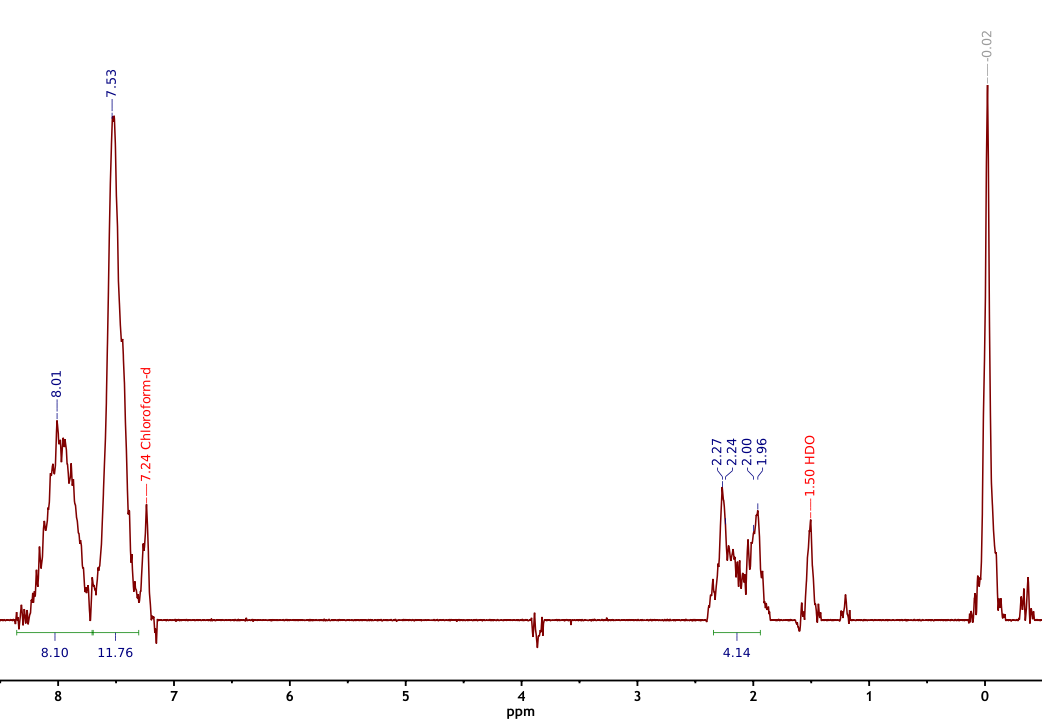
\includegraphics[width=\textwidth]{figures/nidppe_hnmr.png}
	\caption{
		60 MHz \h\ NMR spectrum of \nidppe. The impurities are listed as
		follows (\del): \cite{nmrtable} 7.24 ppm (\cdcl, s), 1.50 ppm
		(HDO, s), $-0.02$ ppm (TMS, s).
	}
\end{figure}

\section{\p\ NMR Spectra}

\subsection{\p\ NMR spectrum of dppe}

\begin{figure}[H]
	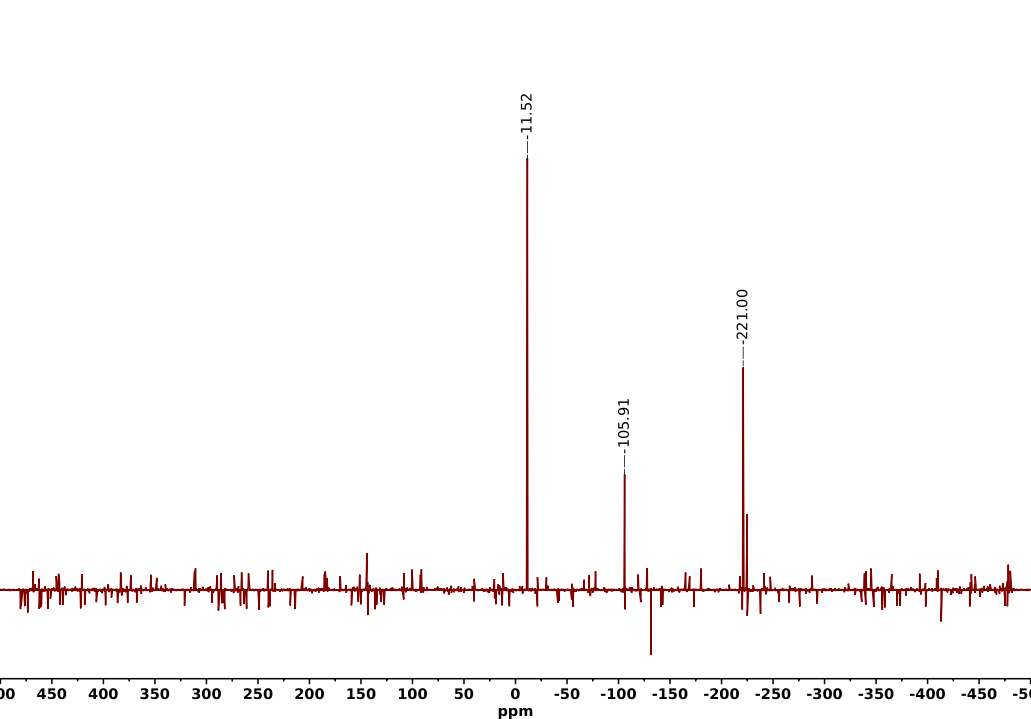
\includegraphics[width=\textwidth]{figures/dppe_pnmr.png}
	\caption{
		400 MHz \p\ NMR spectrum of dppe. Note the instrument artifacts
		at $-105.91$ ppm and $-221.00$ ppm.
	}
\end{figure}

\begin{figure}[H]
	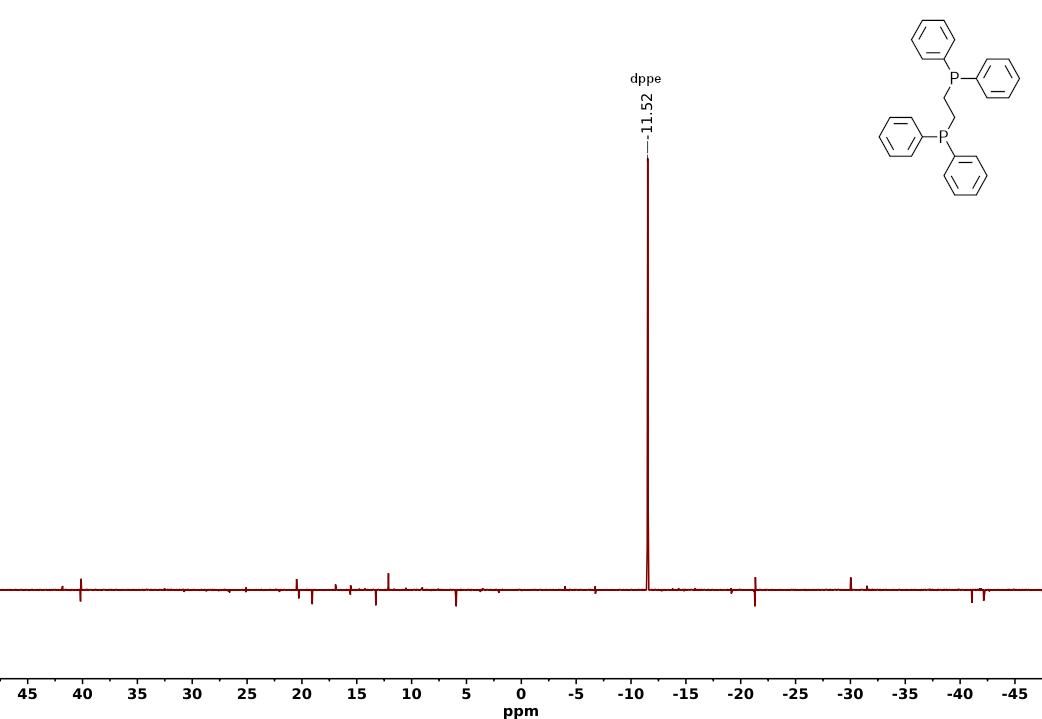
\includegraphics[width=\textwidth]{figures/zoom_dppe_pnmr.png}
	\caption{
		400 MHz \p\ NMR spectrum of dppe, enhanced near the product
		peak.
	}
\end{figure}

\subsection{\p\ NMR spectrum of \nidppe}

\begin{figure}[H]
	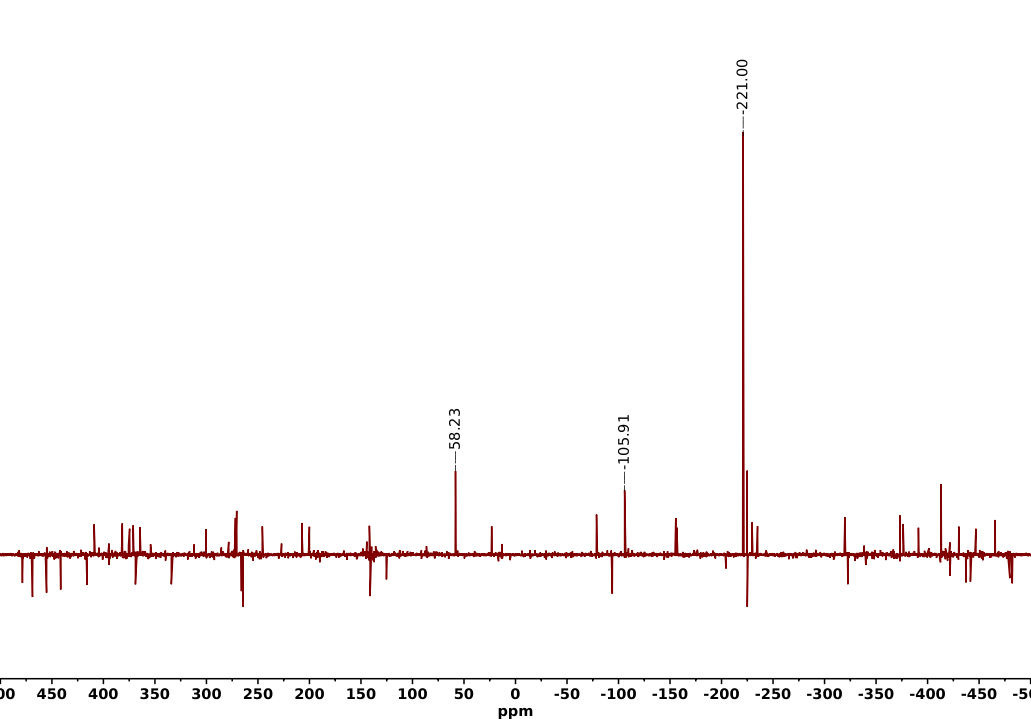
\includegraphics[width=\textwidth]{figures/nidppe_pnmr.png}
	\caption{
		400 MHz \p\ NMR spectrum of \nidppe. Note the instrument
		artifacts at $-105.91$ ppm and $-221.00$ ppm.
	}
\end{figure}


\begin{figure}[H]
	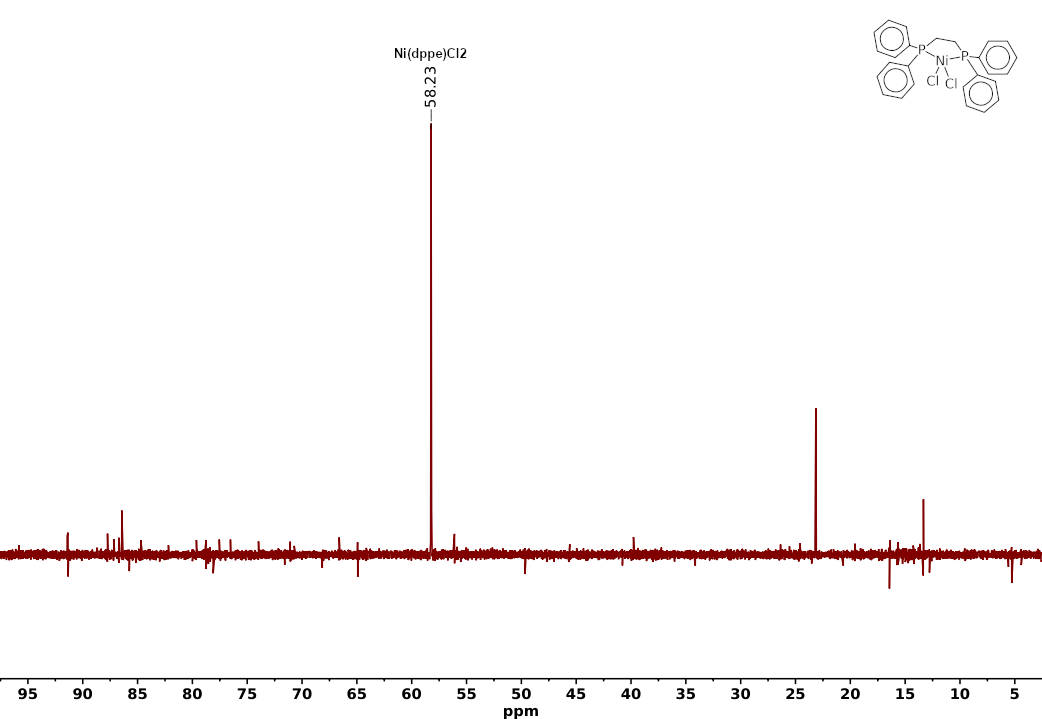
\includegraphics[width=\textwidth]{figures/zoom_nidppe_pnmr.png}
	\caption{
		400 MHz \p\ NMR spectrum of \nidppe, enhanced near the product
		peak.
	}
\end{figure}

\section{IR Spectra}

\subsection{IR spectrum of dppe}

\begin{figure}[H]
	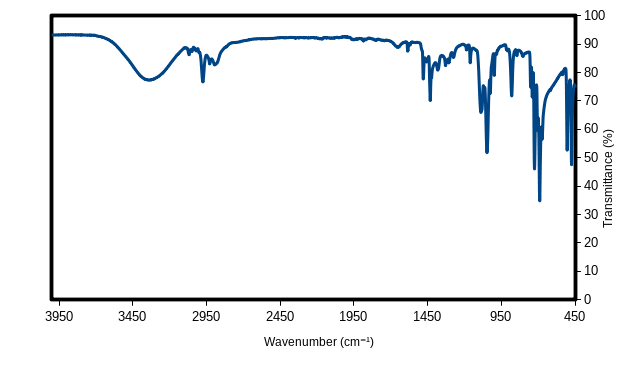
\includegraphics[width=0.8\textwidth]{figures/dppe_ir.png}
	\caption{IR spectrum of dppe. Note the presence of ethanol ($\tilde\nu$ = 3300 \wavenum).}
\end{figure}

\subsection{IR spectrum of \nidppe}

\begin{figure}[H]
	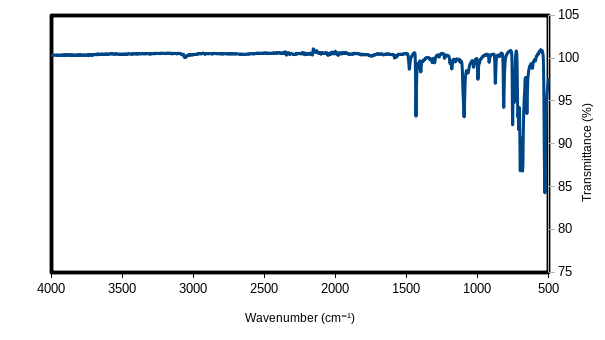
\includegraphics[width=0.8\textwidth]{figures/nidppe_ir.png}
	\caption{IR spectrum of \nidppe.}
\end{figure}

\bibliography{lab_3.bib}

\end{document}
